\documentclass[twoside]{hcmut-report}
\usepackage{codespace}

% Sub-preambles
% https://github.com/MartinScharrer/standalone

% Encodings
\usepackage{gensymb,textcomp}

\usepackage{amsmath,amsfonts,amsthm} % Math packages

\usetikzlibrary{automata, positioning, arrows}

% Better tables
% Wide tables go to https://tex.stackexchange.com/q/332902
\usepackage{array,multicol,multirow,siunitx,tabularx}

% Better enum
\usepackage{enumitem}

% Graphics
\usepackage{caption,float}

% Configurations
\coursename{Prova Finale}
\reporttype{Progetto di Reti Logiche}
\title{Relazione}
\advisor{William Fornaciari}
\author{Simone Corbo}
\studentPersonalCode{10727140}
\studentMatricola{955854}


% Rename some sections
%\AtBeginDocument{\renewcommand*{\contentsname}{Contents}}
%\AtBeginDocument{\renewcommand*{\refname}{References}}
%\AtBeginDocument{\renewcommand*{\bibname}{References}}

% Custom commands
\newcommand*\mean[1]{\bar{#1}}

\tikzset{
%-&gt;,  % makes the edges directed
%&gt;=stealth, % makes the arrow heads bold stealth
    node distance=5cm, % specifies the minimum distance between two nodes. Change if necessary.
    initial text=$\ \ $, % sets the text that appears on the start arrow
}



\begin{document}
    \coverpage

%\section*{Member list \& Workload}
%\newcounter{memberrowno}
%\setcounter{memberrowno}{0}
%\begin{center}
%  \begin{tabular}{>{\stepcounter{memberrowno}\thememberrowno}llcc}
%    \toprule
%    \multicolumn{1}{c}{\textbf{No.}} & \textbf{Full name} & \textbf{Student ID} & \textbf{Contribution} \\
%    \midrule
%                                     & h                  & xxxxxxx             & 100\%                       \\
%                                     & h                  & xxxxxxx             & 100\%                       \\
%    \bottomrule
%  \end{tabular}
%\end{center}
%\clearpage

    \tableofcontents

    \clearpage
    This is how you normally work with \LaTeX, but you can also split a project into smaller files for easier management.
    %To import other files, you can use \mintinline{latex}{\input{}} or \mintinline{latex}{\include{}}.
    There differences can be found at \url{https://tex.stackexchange.com/a/250}, but in short

    %\begin{center}
    %    \mintinline{latex}{\include{filename}} = \mintinline{latex}{\clearpage \input{filename} \clearpage}
    %\end{center}

    \section{Introduzione}



    L'obiettivo non è la ''copia'' della specifica ma una elaborazione, con un esempio e, se è possibile, un disegno e/o una immagine, che spieghi cosa succede;

    La funzione richiesta nella specifica viene realizzata tramite due componenti fondamentali.

    Il primo, denominato DeSerializerTransform (di seguito indicato come DeSerT), si occupa di fare il parsing delle informazioni ricevute in input, ricavando dall'ingresso seriale di input, il numero del canale di output scelto e l'indirizzo nel quale sono salvati i dati in memoria, entrambi salvati in parallelo tramite dei vettori di bit.
    Il suo funzionamento si basa su una macchina a stati finiti, di seguito riportato.

    \begin{figure}[ht]
        \label{FSM2}
        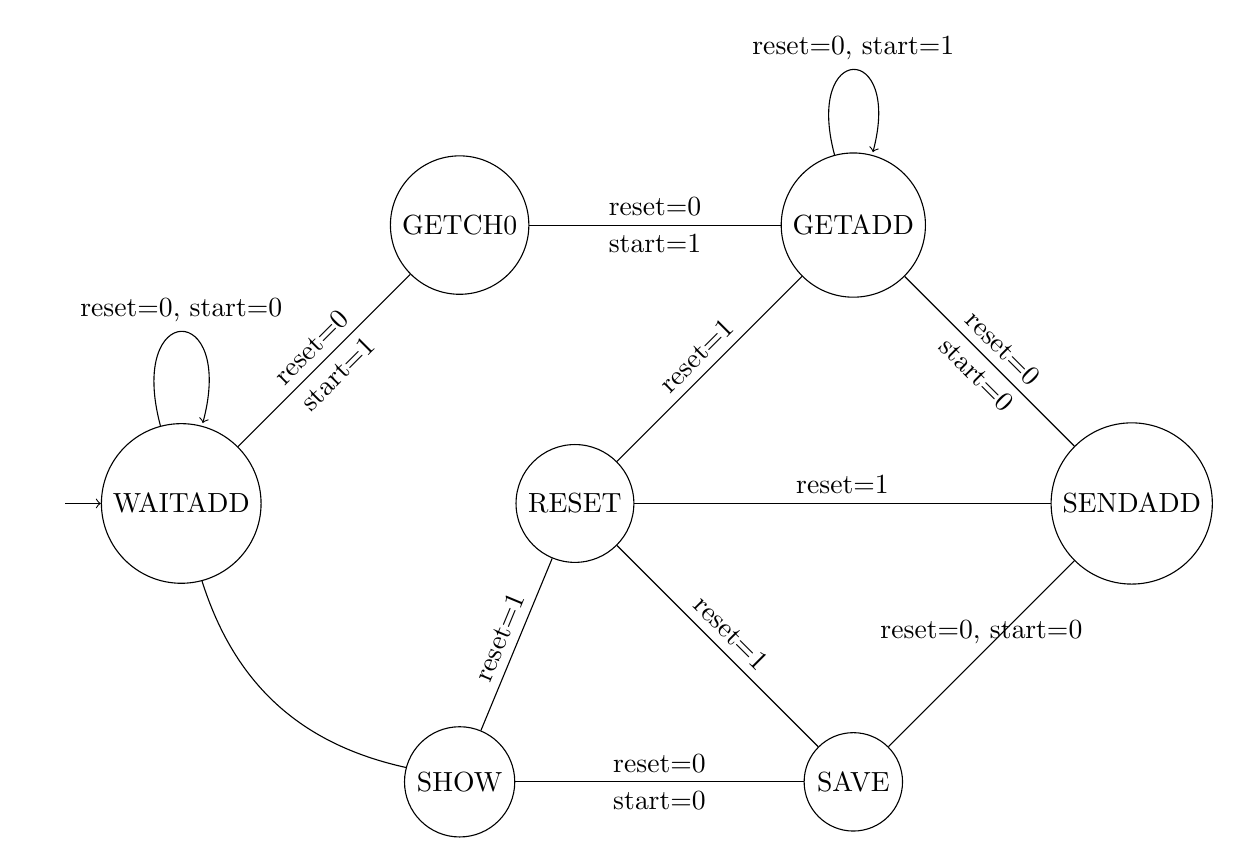
\begin{tikzpicture}
            \node[state, initial] (WAITADD) {WAITADD};
            \node[state, above right of=WAITADD] (GETCH0) {GETCH0};
            \node[state, right of=GETCH0] (GETADD) {GETADD};
            \node[state, below right of=GETADD] (SENDADD) {SENDADD};
            \node[state, below left of=SENDADD] (SAVE) {SAVE};
            \node[state, left of=SAVE] (SHOW) {SHOW};

            \node[state, right of=WAITADD] (RESETs) {RESET};


            \path (WAITADD) edge[loop above] node{reset=0, start=0} (WAITADD)
            (WAITADD) edge[above] node[above, sloped]{reset=0}
            node[below, sloped]{start=1}
            (GETCH0)
            (GETCH0) edge[above] node[above, sloped]{reset=0}
            node[below, sloped]{start=1}(GETADD)
            (GETADD) edge[loop above] node{reset=0, start=1} (GETADD)
            (GETADD) edge[above] node[above, sloped]{reset=0}
            node[below, sloped]{start=0}
            (SENDADD)
            (SENDADD) edge[above] node{reset=0, start=0} (SAVE)
            (SAVE) edge[above] node[above]{reset=0}
                               node[below]{start=0} (SHOW)
            (SHOW) edge[bend left, below] node{} (WAITADD)

            (GETADD) edge[above, sloped] node{reset=1} (RESETs)
            (SENDADD) edge[above, sloped] node{reset=1} (RESETs)
            (SAVE) edge[above, sloped] node{reset=1} (RESETs)
            (SHOW) edge[above, sloped] node{reset=1} (RESETs);



        \end{tikzpicture}
    \end{figure}

    La lunghezza dei dati in input è variabile, tra 2 e 18 bit, ma lo schema dei dati è costante, perché i primi 2 bit rappresentano sempre il canale (da 00 a 11), mentre i restanti rappresentano l'indirizzo di memoria



    Mentre il secondo si occupa di inserire i dati nel canale corretto e gestisce la corretta visualizzazione dei dati.



    \begin{figure}[ht]
        \label{FSM}
        \begin{tikzpicture}
            \node[state, initial] (q1) {$q_1$};
            \node[state, right of=q1] (q2) {$q_2$};
            \node[state, right of=q2] (q3) {$q_3$};
            \draw (q1) edge[loop above] node{0} (q1)
            (q1) edge[above] node{1} (q2)
            (q2) edge[loop above] node{1} (q2)
            (q2) edge[bend left, above] node{0} (q3)
            (q3) edge[bend left, below] node{0, 1} (q2);
        \end{tikzpicture}
    \end{figure}

    \section{Architettura}
    L’obiettivo è quello di riportare un schema funzionale (lo schema in moduli... un bel disegno chiaro... i segnali i bus, il/i clock, reset... );
    \subsection{Modulo 1}
    (la descrizione - sottoparagrafo - di ogni modulo e la scelta
    implementativa - per esempio, il modulo ... è una collezione di process che
    implementano la macchina a stati e la parte di registri, .... La macchina a stati,
    il cui schema in termini di diagramma degli stati, ha 8 stati. Il primo
    rappresenta .... e svolge le operazioni di ... il secondo... etc etc)
    \subsection{Modulo ...}

    \section{Risultati sperimentali}

    \subsection{Sintesi (Report di sintesi)}
    \label{subsec:report}
    \subsection{Simulazioni}
    \label{subsec:sim}
    L'obiettivo non è solo riportare i risultati ottenuti attraverso la
    simulazione test bench forniti dai docenti, ma anche una analisi personale e
    una identificazione dei casi particolari; il fine è mostrare in modo convincente
    e più completo possibile, che il problema è stato esamintato a fondo e che,
    quanto sviluppato, soddisfa completamente i requisiti.
    i. test bench 1 (cosa fa e perchè lo fa e cosa verifica; per esempio,
    controlla una condizione limite)
    ii. test bench 2 (....)
    4. conclusioni (mezza pagina max




    \section{Better tables}
The recommended way is by using the booktabs package and drop all vertical rules.

Tabularx is simply tabular but with X environment, meaning that it will try to use all of \mintinline{latex}{\linewidth}.

\begin{center}
    \begin{tabularx}{\linewidth}{l*{2}{X}}
        \toprule
        & OOP & FP \\
        \cmidrule(lr){2-3}
        Pros &     &    \\
        &     &    \\
        &     &    \\
        \midrule
        Cons &     &    \\
        &     &    \\
        &     &    \\
        \bottomrule
    \end{tabularx}
\end{center}

More information can be found at \url{https://latex-tutorial.com/tables-in-latex/}.

    \section{Better enumerator}
Normal enumerator gets the job done, but what if you want custom numbering?
This implementation allows custom labeling, either by pre-defined rules or in-place.

\begin{enumerate}[label={\alph*.yeah}]
    \item First item
    \item Second item
    \item[custom] Third item
\end{enumerate}

    \section{Codeblocks}
There are several ways to embed code in a \LaTeX{} file.
Here are inline code, embedded codeblock, and external import.

\begin{itemize}
    \item External import

    \inputcode[highlightlines={1,10-13}]{Python}{code/example.py}

    \item With custom line range

    \inputcode[firstline=10,lastline=13]{Python}{code/example.py}

    \item Embedded

    \begin{code}{Python}
  class iostream:
      def __lshift__(self, other):
          print(other, end='')
          return self

      def __repr__(self):
          return ''
    \end{code}

    \item Inline

    \mintinline{Python}{print('Hello, world!')}
\end{itemize}

You can also define your custom inline as \url{https://tex.stackexchange.com/a/148479}.

This is one way to input algorithms.

\begin{algorithm}[H]
    \caption{QL algorithm}
    Initialize \(Q\)-table values \((Q(s, a))\) arbitrarily\;
    Initialize a state \((s_t)\)\;
    Repeat Steps~\ref{alg:step_4} to~\ref{alg:step_6} until learning period ends\;
    Choose an action \((a_t)\) for the current state \((s_t)\) using an exploratory policy\; \nllabel{alg:step_4}
    Take action \((a_t)\) and observe the new state \((s_t + 1)\) and reward \((r_t + 1)\)\;
    Update \(Q\)-value\; \nllabel{alg:step_6}
\end{algorithm}


    \bibliographystyle{plain}
    \bibliography{refs/example.bib}
    \nocite{*}

\end{document}
